%This template is a modification of the templated made by Rob Rutten found at http://www.staff.science.uu.nl/~rutte101/rrweb/rjr-edu/manuals/student-report/

%%%%%%%%%%%%%%%%%%%%%%%%%%%%%%%%%%%%%%%%%%%%%%%%%%%%%%%%%%%%%%%%%%%%%%%%%%%%
%\documentclass{aa}   %% Astronomy & Astrophysics style class
\documentclass[a4paper]{article}
\usepackage{geometry}
\geometry{a4paper}
\usepackage{subcaption}
\usepackage{graphicx,url,twoopt}
%\usepackage{biblatex}
\usepackage{enumitem}
\usepackage{amsmath}
\usepackage[varg]{txfonts}           %% A&A font choice
%\usepackage{hyperref}                %% for pdflatex
%%\usepackage[breaklinks]{hyperref}  %% for latex+dvips
%%\usepackage{breakurl}              %% for latex+dvips
%\usepackage{pdfcomment}              %% for popup acronym meanings
%\usepackage{acronym}                 %% for popup acronym meanings
\usepackage{calrsfs}
\DeclareMathAlphabet{\pazocal}{OMS}{zplm}{m}{n}

\usepackage{natbib}
% \hypersetup{
%   colorlinks=true,   %% links colored instead of frames
%   urlcolor=blue,     %% external hyperlinks
%   linkcolor=red,     %% internal latex links (eg Fig)
%}
%\bibpunct{(}{)}{;}{a}{}{,}    %% natbib cite format used by A&A and ApJ
%\pagestyle{plain}   %% undo the fancy A&A pagestyle 

%%%%%%%%%%%%%%%%%%%%%%%%%%%%%%%%%%%%%%%%%%%%%%%%%%%%%%%%%%%%%%%%%%%%%%%%%%%%
\begin{document}  
%\twocolumn[{%
\vspace*{4ex}
\begin{center}
  {\Large \bf Compulsory exercise STK4900 Spring 2016}\\[4ex]
  {\large \bf Andreas Ellewsen$^1$}\\[4ex]
  \begin{minipage}[t]{15cm}
        $^1$ Institute of Theoretical Astrophysics, University of Oslo, P.O. Box 1029 Blindern, N-0315 Oslo, Norway\\
                     
    {\bf Abstract.} I use data from two different studies. One to draw conclusions on whether the number of cars present in some geographical area has any influence on the concentration of NO2 in that same area. And another to decide whether or not treating patients suffering from liver cirrhosis with prednisone has an effect.
    
  \vspace*{2ex}
  \end{minipage}
\end{center}
%}]

%%%%%%%%%%%%%%%%%%%%%%%%%%%%%%%%%%%%%%%%%%%%%%%%%%%%%%%%%%%%%%%%%%%%%%%%%%%%
\section{Introduction}\label{sec:introduction}
%%%%%%%%%%%%%%%%%%%%%%%%%%%%%%%%%%%%%%%%%%%%%%%%%%%%%%%%%%%%%%%%%%%%%%%%%%%%
This report consist of two parts. 

The first part uses data from a measuring station at Alnabru in Oslo. This data contains meteorological measurements, traffic volume, and air pollution. The air pollution is measured using the concentration of NO$_2$ particles in the air.
This purpose of this study is to look for a connection between the number of cars and the air pollution in the area.

The second part studies a dataset containing 488 patients with liver cirrhosis who have been included in a randomized clinical trial. This dataset contains various medical measurements like gender, age, and time from start of treatment until death. The purpose of the study was to investigate whether or not prednisone had an effect on the survival of the patients. Of the 488 patients, 251 of the patients received prednisone, and 237 received a placebo. 

To study the datasets I have chosen to use the programming language R. This is a language that works exceptionally well for statistical analysis.

%%%%%%%%%%%%%%%%%%%%%%%%%%%%%%%%%%%%%%%%%%%%%%%%%%%%%%%%%%%%%%%%%%%%%%%%%%%%
\section{Traffic and air pollution}\label{sec:Equations}
%%%%%%%%%%%%%%%%%%%%%%%%%%%%%%%%%%%%%%%%%%%%%%%%%%%%%%%%%%%%%%%%%%%%%%%%%%%%
The variables in the dataset are 
\begin{itemize}
 \item{\makebox[2cm]{\bf no2\hfill}The logarithm of the concentration of NO$_2$}
 \item{\makebox[2cm]{\bf log.cars\hfill}The logarithm of the number of cars per hour}
 \item{\makebox[2cm]{\bf temp\hfill}Temperature 2 meters above the ground (degrees C)}
 \item{\makebox[2cm]{\bf wind.speed\hfill}Wind speed (meters/second)}
 \item{\makebox[2cm]{\bf hour.of.day\hfill}Hour of the day the measurements were collected (1-24)}
\end{itemize}
The purpose of the study is to find an explanation for the levels of air pollution. The obvious choice to explain this is the number of cars present. Because of this we make some summaries of the data for these variables in tables \ref{NO2} and 
\ref{log.cars}.

\begin{table}
\begin{center}
\begin{tabular}{|c|c|c|c|c|c|}
   \hline
   NO$_2$&&&&&\\
   \hline
   Min &1st Qu. & Median& Mean & 3rd Qu. & Max\\
   \hline
   1.224 & 3.214 & 3.848 & 3.698 & 4.217 & 6.395\\
   \hline
 \end{tabular}
 \caption{Summary of the NO$_2$ data.}
 \label{NO2}
\end{center}
\end{table}

\begin{table}
\begin{center}
\begin{tabular}{|c|c|c|c|c|c|}
   \hline
   log.cars&&&&&\\
   \hline
   Min &1st Qu. & Median& Mean & 3rd Qu. & Max\\
   \hline
  4.127 & 6.176 & 7.425&  6.973 & 7.793 & 8.349 \\
   \hline
 \end{tabular}
 \caption{Summary of the logarithm of cars.}
 \label{log.cars}
\end{center}
\end{table}
The information in tables \ref{NO2} and \ref{log.cars} may be easier to study with a box plot (see fig \ref{boxno2logcars}).

\begin{figure}
\begin{subfigure}{.5\textwidth}
 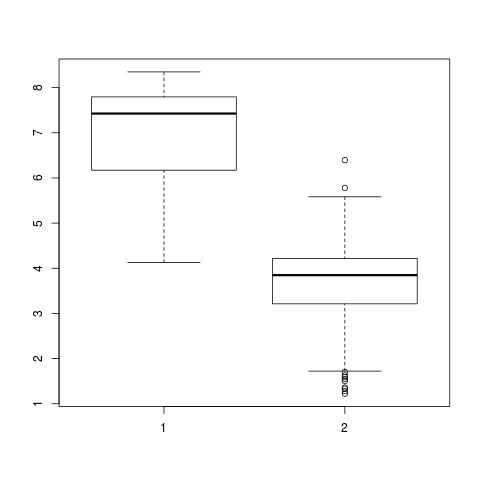
\includegraphics[width=\textwidth]{boxno2logcars.png}
 \caption{Boxplot with the logarithm of the number of cars as 1, and concentration of NO$_2$ as 2.}
 \label{boxno2logcars}
 \end{subfigure}
 \begin{subfigure}{.5\textwidth}
  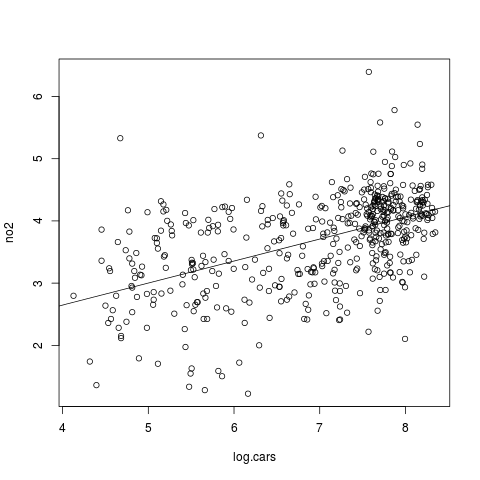
\includegraphics[width=\textwidth]{no2_v_logcars.png}
 \caption{The plot shows the concentration of NO$_2$ as a function of the logarithm of cars. A linear fit to this data indicates that there is a correlation between the two.}
 \label{no2cars}
 \end{subfigure}
 \caption{}
 \end{figure}  
To see if there is a correlation between these two variables we plot NO$_2$ as a function of the logarithm of the number of cars. We then fit a linear regression model to the data. The results can be seen in figure \ref{no2cars}. The line is of the form $y = ax + b$. Here $a = 0.3535$, and $b = 1.2331$. This tells us that the average NO$_2$ is $0.3535$ if there are no cars present, and that if logarithm of the number of cars increases by $1$, the NO$_2$ concentration increases by $0.3535$. 

Calculating the Pearson Correlation Coefficient results in $r = 0.5120504$. Since we are using linear regression we can square this to get the coefficient of determination $R^2 = 0.2622$. This tells us how close the measurements are to the model. (Perfect positive correlation gives $R^2 = 1$, while perfect negative correlation gives $R^2 = -1$.)

In this case $R^2$ is quite low, indicating that we should include more explanatory variables. Making a plot of all the variables as functions of each other should make it easier to spot obvious correlations.

Looking at figure \ref{alldata} we spot the correlation we have already tested on the top row to the left (NO$_2$ vs log(cars) ). Using temperature as an explanatory variable results in a blob which looks seemingly random. However, wind speed seems like it could be negatively correlated, and time of day seems positively correlated. 
Testing correlations between all variables returns table \ref{tablealldata}.

\begin{figure}[ht]
 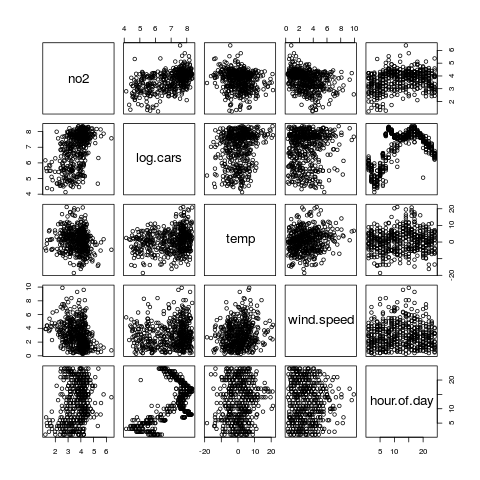
\includegraphics[width=.99\textwidth]{alldata.png}
 \caption{The figures shows all the variables as functions of each other. The ones we are interested in are the top row. Namely NO$_2$ as functions of the others.}
 \label{alldata}
\end{figure}

\begin{table}[ht]
\begin{center}
\begin{tabular}{|c|c|c|c|c|c|}
   \hline
   &NO$_2$&log(cars)&temp&wind.speed&hour.of.day\\
   \hline
   NO$_2$&1.0000000 &0.51205042& -0.1681592 &-0.328834938 & 0.246201259\\
   \hline
   log(cars)&0.5120504 &1.00000000 & 0.2018317 & 0.097530682 & 0.576856715\\
   \hline
   temp&-0.1681592& 0.20183175 & 1.0000000 & 0.165990712 & 0.079484997\\
   \hline
   wind.speed&-0.3288349 &0.09753068 & 0.1659907 & 1.000000000 &-0.002789753\\
   \hline
   hour.of.day&0.2462013 &0.57685671 & 0.0794850 &-0.002789753 & 1.000000000\\
   \hline
 \end{tabular}
\end{center}
 \caption{Correlations between all the variables in the data set.}
 \label{tablealldata}
\end{table}
Looking at the values there does seem to be at least some correlation between NO$_2$ and all the others. We should be careful though. We do not want to include too many variables. Looking at the rest of the table reveals that there are som correlations between other variables as well. 

Hour of day is correlated to the number of cars, which is obvious when considering that people work in shifts. Looking at the figure reveals that it is the people who work the day shift that dominate the data.
The number of cars is also correlated to the temperature. So more people are driving when it is warm outside.
It is also correlated to the wind speed. This connection is not immediately obvious.
Considering temperature, we see that there is a correlation between it and wind speed. Heat causes the air to rise, which could contribute to this. This could explain why the number of cars was correlated to the wind speed.
Surprisingly, the temperature is not strongly correlated to the hour of day, which one would expect.
Finally, the hour of the day is not correlated to the wind speed.	
From this it is clear that there are correlations between the explanatory variables. This means that one variable could explain some portion of the correlation between another variable and the concentration NO$_2$.
Thus we should include all the variables in the model, and then eliminate as many as possible, while keeping those that give a a large contribution to $R^2$.
The first attempt is to make a model using a model of the form

\begin{equation}
\begin{aligned}
y  &= A + BT + Clog(n_c)+ Dw + Eh + FT^2 + Glog^2(n_c) \\
   &+ Hw^2 + Ih^2 +Jlog(w)+Klog(h)+Llog^2(w)+Mlog^2(h)
\end{aligned}
\end{equation}
where $A,B,C,D,E,F,G,H,I,J,K,L,M$ are constants, $T$ temperature, $n_c$ number of cars, $w$ wind speed, and $h$ hour of day.

This is a good example of a terrible model. Note that we could make this even worse by bringing in exponentials and roots. I have also chosen to not include interactions. Even so this will work well as a starting point.
The next step is to keep removing terms that are unnecessary until we have a simple model which can explain a large portion of the data. 

Running the summary function in R on this model returns $R^2 = 0.5104$, and the adjusted $R^2 = 0.4983$. 
The summary also shows that most of the variables contribute very little to the precision of the model.
We remove the worst ones and end up with the following model:

\begin{equation}
\begin{aligned}
y  &= A + BT + Clog(n_c)+ Dw + Eh + FT^2 + Glog^2(n_c) \\
   &+ Jlog(w)+Klog(h)+Llog^2(w)+Mlog^2(h)
\end{aligned}
\end{equation}
This one has $R^2 = 0.5103$, and adjusted $R^2=0.5003$. Note that the adjusted $R^2$ has increased. We should keep going.
We remove even more terms with little significance ending up with 
\begin{equation}
\begin{aligned}
y  &= A + BT + Dw + Eh + Glog^2(n_c) \\
   &+Jlog(w)+Klog(h)+Llog^2(w)+Mlog^2(h)
\end{aligned}
\end{equation}
Now $R^2=0.5084$, and adjusted $R^2=0.5004$. The adjusted one keeps increasing.	
The next model is 
\begin{equation}
\begin{aligned}
y  &= A + BT + Dw + Glog^2(n_c) \\
   &+Jlog(w)+Llog^2(w)+Mlog^2(h)
\end{aligned}
\end{equation}
This is the first time the adjusted $R^2$ decreases to $R^2= 0.4968$. For reference $R^2 = 0.5029$. Now one might be tempted to stop removing terms since the adjusted $R^2$ has started decreasing and this works as a guide for when to stop adding more terms, indicating that our last model was better. I choose to keep removing more terms since the decrease is not very significant yet.
This brings us to
\begin{equation}
\begin{aligned}
y  &= A + BT + Dw + Glog^2(n_c) \\
   &+Jlog(w)+Llog^2(w)
\end{aligned}
\end{equation}
with $R^2 = 0.495$ and adjusted $R^2 = 0.4899$. The decrease is still not significant.

Removing one more term gives
\begin{equation}
\begin{aligned}
y  &= A + BT + Glog^2(n_c) \\
   &+Jlog(w)+Llog^2(w)
\end{aligned}
\end{equation}
This is starting to look like a fairly simple model. However the last term is not significant for the model so we will remove it and get our final model:
\begin{equation}
y = A + BT + Clog^2(n_c) + Dlog(w)
\end{equation}
with $A=2.518597$, $B=-0.026630$, $C=0.031874$, $D=-0.418826$.
This model has $R^2=0.4846$ and adjusted $R^2=0.4804$.
Interpreting this model, $A$ is the logarithm of the concentration of $NO_2$ if $T=log^2(n_c)=log(w)=0$. $B$, $C$, and $D$ are the respective increases if the corresponding terms were to grow by 1. (e.g $B$ is the increase if $log^2(n_c)$ increased by 1.)

With all the numbers inserted we have
\begin{equation}
y = 2.518597 - 0.026630T + 0.031874log^2(n_c) - 0.418826log(w).
\end{equation}
For conclusions regarding this model see section \ref{sec:conclusions}
%%%%%%%%%%%%%%%%%%%%%%%%%%%%%%%%%%%%%%%%%%%%%%%%%%%%%%%%%%%%%%%%%%%%%%%%%%%%
\section{Prednisone and survival}\label{sec:Imp}
%%%%%%%%%%%%%%%%%%%%%%%%%%%%%%%%%%%%%%%%%%%%%%%%%%%%%%%%%%%%%%%%%%%%%%%%%%%%
The variables in the dataset are 
\begin{itemize}
 \item{\makebox[2cm]{\bf status\hfill}Indicator for death/censoring (1=dead; 0=censored)}
 \item{\makebox[2cm]{\bf time\hfill}Time in days from start of treatment to death/censoring}
 \item{\makebox[2cm]{\bf treat\hfill}Treatment (0=prednisone; 1=placebo)}
 \item{\makebox[2cm]{\bf sex\hfill}Gender (0=female; 1=male)}
 \item{\makebox[2cm]{\bf asc\hfill}Ascites at start of treatment (0=none; 1=slight; 2=marked)}
 \item{\makebox[2cm]{\bf age\hfill}Age in years at start of treatment}
 \item{\makebox[2cm]{\bf agegr\hfill}Age group (1=<50; 2=50-65; 3=>65)}
\end{itemize}

The first step is to make Kaplan-Meier plots for the survival function for each level of the covariates
treatment, sex, ascites, and grouped age. 

The resulting plots can be seen in figures \ref{asc},\ref{sex},and \ref{treat}.


\begin{figure}
 \begin{subfigure}{.5\textwidth}
  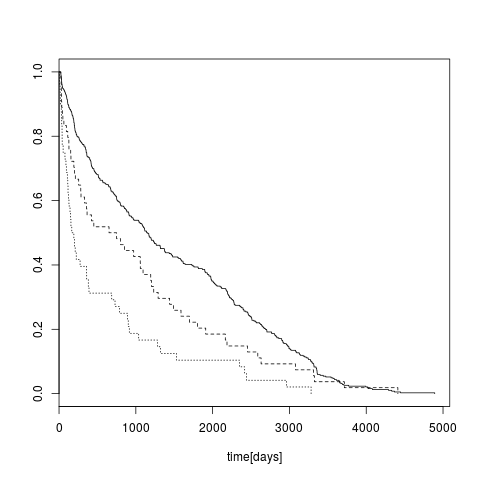
\includegraphics[width=\textwidth]{asc.png}
  \caption{Survival curves for grades of ascites. Solid = none, dashed=slight, dotted = marked.}
  \label{asc}
 \end{subfigure}
 \begin{subfigure}{.5\textwidth}
  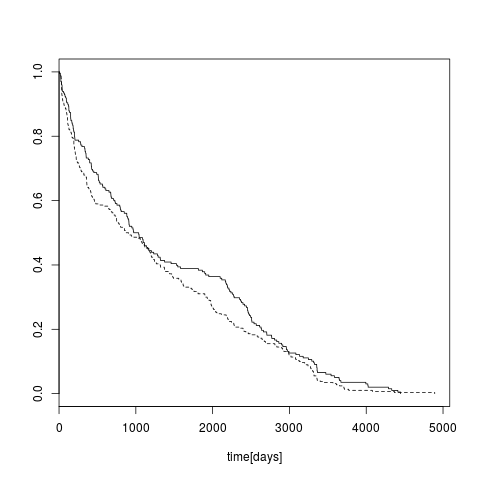
\includegraphics[width=\textwidth]{sex.png}
  \caption{Survival curves for different sex. Solid = female, dashed = male.}
  \label{sex}
 \end{subfigure}
 \begin{subfigure}{.5\textwidth}
  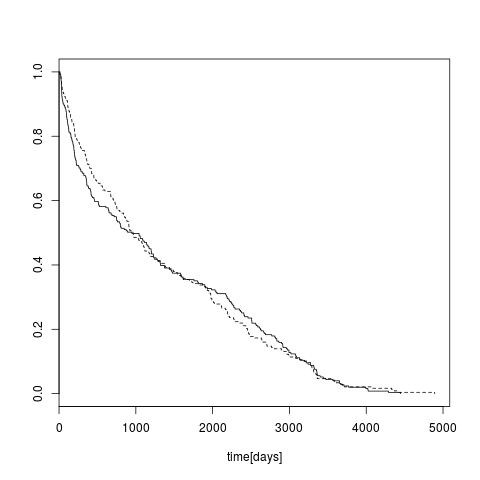
\includegraphics[width=\textwidth]{treat.png}
  \caption{The survival curves for those treated and those not. Solid = treated, dashed = placebo.}
  \label{treat}
 \end{subfigure}
\end{figure}  


Visually one may say that treatment, and sex seem be insignificant. While ascites, and age group are significant

It would be nice to have some numbers describing the significance of the various covariates. 
For this we use the log-rank test. The log-rank test checks if there is a difference between two or more survival curves. In our case we look at the difference between those treated, and those not. 

The results for the different tests can be seen in table \ref{log-rank}. It becomes clear straight away that treatment is not significant, while sex, ascites and age group are. 

\begin{table}[ht]
\begin{center}
\begin{tabular}{|l|l|}
   \hline
   Covariate&p-value\\
   \hline
   Treatment&$0.924$\\
   \hline
   Sex&$0.0984$\\
   \hline
   Ascites&$1.64\times10^{-9}$\\
   \hline
   Age group&$3.86\times10^{-6}$\\
   \hline
 \end{tabular}
\end{center}
 \caption{Results from the log-rank test. Low p-values indicate high significance of the covariate on the survival time.}
 \label{log-rank}
\end{table}

To study this further I do multiple cox regression. The model predicts survival as a function of treatment, sex, ascites, and age. Here age is no longer age group, but instead actual age of the patients. I do not include censored results.

This means that our model is
\begin{equation}
 \lambda(t|X_i) = \lambda_0\exp(\beta_1 X_{1i}+ \beta_2 X_{2i} + \beta_3 X_{3i} + \beta_4 X_{4i}),
\end{equation}
with $beta_k$ corresponding to 1 unit increase in $X_{ki}$. For our model $X_{1i} = 0$ means the subject was not treated, while $X_{1i} = 1$, means he/she was. The other X's work the same way. 

We should study the effects individually. Let us start with the difference between men and women.

Keeping all other covariates constant, the risk ratio for men compared to women is $\exp(\beta_2)=\exp(0.46) = 1.59$. This indicates that the risk of death increases by approximately $60\%$ when looking at men compared to women. This has a confidence interval $[1.24 , 2.03]$, so the odds are somewhere between $24\%$ and $103\%$ worse for men. 

This model includes treatment which we found was not significant. This is still the case so I remove that. We should also check for interactions. 
For those familiar with R, our model is now 
\begin{verbatim}
coxfit.3=coxph(Surv(time,status==1)~sex+asc+age+sex:age+sex:asc+asc:age,data=cirrhosis)
\end{verbatim}
and running the summary command in R on this model returns
\begin{verbatim}
R output (edited)
             coef exp(coef)  se(coef)      z Pr(>|z|)   
sex     -1.335185  0.263110  0.840774 -1.588  0.11228   
asc      0.389508  1.476254  0.596933  0.653  0.51407   
age      0.033191  1.033748  0.011041  3.006  0.00265 **
sex:age  0.027578  1.027962  0.013524  2.039  0.04144 * 
sex:asc  0.197581  1.218452  0.172422  1.146  0.25183   
asc:age  0.001863  1.001865  0.008786  0.212  0.83207   

Concordance= 0.683  (se = 0.019 )
Rsquare= 0.21   (max possible= 0.999 )
Likelihood ratio test= 115.3  on 6 df,   p=0
Wald test            = 128.1  on 6 df,   p=0
Score (logrank) test = 147.4  on 6 df,   p=0
\end{verbatim}
From this the rest is simple elimination, of the terms that are insignificant. The obvious choice is the interaction between ascites and age. Continuing with the next model, we see that the interaction between sex and ascites is not significant so that is removed. The next run reveals that the least significant covariate is sex with $p = 0.10$. This is still larger than $5\%$ which is the general limit used so this is removed.

Our final model is then the one which includes ascites,age, and the interaction between sex and age.
The output of the final model is included for reference:
\begin{verbatim}
 R output (edited):
coxph(formula = Surv(time, status == 1) ~ asc + age + sex:age, 
    data = cirrhosis)
            coef exp(coef) se(coef)     z Pr(>|z|)    
asc     0.605325  1.831847 0.082971 7.296 2.97e-13 ***
age     0.044587  1.045595 0.006658 6.696 2.14e-11 ***
age:sex 0.007888  1.007919 0.001980 3.985 6.76e-05 ***

        exp(coef) exp(-coef) lower .95 upper .95
asc         1.832     0.5459     1.557     2.155
age         1.046     0.9564     1.032     1.059
age:sex     1.008     0.9921     1.004     1.012

Concordance= 0.681  (se = 0.019 )
Rsquare= 0.204   (max possible= 0.999 )
Likelihood ratio test= 111.3  on 3 df,   p=0
Wald test            = 118.3  on 3 df,   p=0
Score (logrank) test = 124.9  on 3 df,   p=0
\end{verbatim}


From this we read that the dominating effect on survival is whether or not the patient has ascites. Recall also that there are two grades of the severity of ascites, so even if the patient has just slight ascites at the start of treatment the risk increases by $83\%$. If the patient has marked ascites the risk ratio is $RR = \exp(2\times0.605325)=3.355665$ meaning the risk increases by $236\%$. 
We can also read that the risk increases by $4.6\%$ for women when aging by one year, while men have to take into account the interaction which increases the risk by $0.8\%$. 
%%%%%%%%%%%%%%%%%%%%%%%%%%%%%%%%%%%%%%%%%%%%%%%%%%%%%%%%%%%%%%%%%%%%%%%%%%%%
\section{Conclusions} \label{sec:conclusions}
%%%%%%%%%%%%%%%%%%%%%%%%%%%%%%%%%%%%%%%%%%%%%%%%%%%%%%%%%%%%%%%%%%%%%%%%%%%%
\subsection{Traffic and air pollution}
We observed that increasing temperature reduced the concentration of NO$_2$ in the air. So did increasing wind speed. Unsurprisingly, increasing the number of cars present increased the concentration of NO$_2$. 
It is hard to say how precisely temperature affects the concentration. One conclusion could be that cars pollute less when the temperature is higher. Maybe there is some other source of pollution that slows down when the temperature rises.
The same goes for wind speed. It may be the case that higher wind speed just means that the pollution is blown away to somewhere else. One could also draw the conclusion that higher wind speed makes cars pollute less but that seems strange from a physical standpoint. 
Nevertheless, the conclusion that can be drawn is that if one wants to reduce the level of air pollution in the area one should start by reducing the number of cars.

\subsection{Prednisone and survival}
From the study we found that prednisone had no significant effect on the patients treated. However it was observed that the grade of ascites was highly significant for the survival rate of the patients. Slight ascites increased risk of death by $83\%$, while marked ascites increased it by a staggering $236\%$. 

It was also observed that the age of the patients was significant to the survival rate. For men the risk was increased further which was observed because of the interaction term in the model.

Unless there is some other treatment that has a chance of curing the patients completely one may want to focus on how to reduce the ascites since that has such a large impact on the survival time.
%%%%%%%%%%%%%%%%%%%%%%%%%%%%%%%%%%%%%%%%%%%%%%%%%%%%%%%%%%%%%%%%%%%%%%%%%%%%
\end{document}